Unlike the statistical models presented in the previous sections, XGBoost (Extreme Gradient Boosting) is a machine learning method that makes no parametric assumptions about the underlying data generating process. Where ARIMA models temporal dependence explicitly through autoregressive and moving average components, and OLS assumes a fixed linear relationship between features and the target, XGBoost learns complex non-linear interactions directly from data by sequentially fitting an ensemble of decision trees, each correcting the residual errors of the previous one. \\

A key practical distinction from the models presented earlier is that XGBoost is data-hungry. Cell-specific models, as applied in the ARIMA and OLS sections, operate on a single time series at a time and are therefore well suited to small, isolated datasets. XGBoost however benefits substantially from volume and diversity of training examples. For this reason, all cells across all sites are pooled into a single dataset, allowing the model to learn shared patterns across the entire network simultaneously. \\
This global training approach also changes how cell identity is handled. Rather than fitting a separate model per cell, the cell and site are included as encoded input features, allowing the model to naturally condition its predictions on cell-specific behavior where such structure exists in the data. If a particular cell or site exhibits a distinct traffic pattern, the model will capture this through its learned splits without requiring explicit pre-classification into seasonal and non-seasonal groups as was necessary for the statistical approaches. \\

\subsubsection{Decision tree}
A decision tree works by repeatedly splitting the data based on a single feature and threshold at a time. There is no linearity involved — the model does not assign weights to features or assume any functional form. It simply partitions the feature space into regions, and every observation that falls into the same region receives the same prediction. A single tree of this kind is a very crude approximation, and in practice a single tree tends to overfit easily. \\

Random forests address this by training many trees independently on random subsets of the data and features, a technique known as bootstrapping, and averaging their predictions. This reduces variance and makes the model considerably more robust than any individual tree. \\
XGBoost follows the same principle of combining many trees, but rather than training them independently, it builds them sequentially. Each new tree is fitted to the errors left by all previous trees, so the ensemble improves iteratively rather than by averaging. The final prediction is the sum of all trees: 
\[
\hat{y}_i = \sum_{k=1}^{K} f_k(\mathbf{x}_i)
\]
This approach is known as gradient boosting, and XGBoost is a highly optimised implementation of it that has become one of the most widely used models in applied machine learning. \\

\subsubsection{Implementation}
Since XGBoost processes one observation at a time and has no built-in notion of time or sequential order, it cannot look back at past values the way ARIMA does. This makes feature engineering particularly important. All temporal context that the model needs to understand historical behaviour must be explicitly constructed and provided as input features. With this in mind, the feature set was designed to capture both temporal patterns and cell-specific characteristics, and can be grouped into the following categories. \\

\textbf{Raw network metrics} were included directly from the dataset, covering downlink and uplink data volumes, PRB utilisation, active UEs, throughput, and SINR measurements. These provide the model with direct signal about the current network state. \\

\textbf{Lag features} capture historical values of the target at fixed time offsets: 1, 8, 24, 168, and 720 hours back. These allow the model to condition its prediction on recent observations as well as patterns from the same hour yesterday, the same day last week, and the same period last month.
\textbf{Rolling statistics} were computed across a wide range of windows: 3, 6, 12, 24, 48, 168, 336, 720, and 2160 hours. For each window, the mean, maximum, minimum, and standard deviation were included. This gives the model a rich view of both short-term fluctuations and long-term trends. \\

\textbf{Calendar features} were one-hot encoded to allow the model to learn non-linear patterns tied to time. This includes the hour of the day (0--23), day of the week (0--6), and month of the year (1--12), as well as binary indicators for weekends and public holidays. \\
\textbf{Cell and technology features} were included to allow the model to differentiate between cells. The site group and technology generation (4G/5G) were one-hot encoded, along with the frequency band, covering LTE800, LTE1800, LTE2600, NR700, and NR3500. A binary seasonal indicator was also included based on the pre-classification described in earlier sections.\\

In total this results in \textbf{107 input features} per observation. \\

\subsubsection{XG Boost Results}

The model was trained with 200 trees, a learning rate of 0.05, and a maximum tree depth of 4. The data was split chronologically with 80 percent used for training and 20 percent held out for testing. The final model achieved an RMSE of 1.70 on the test set. \\

\begin{figure}[H]
	\centering
	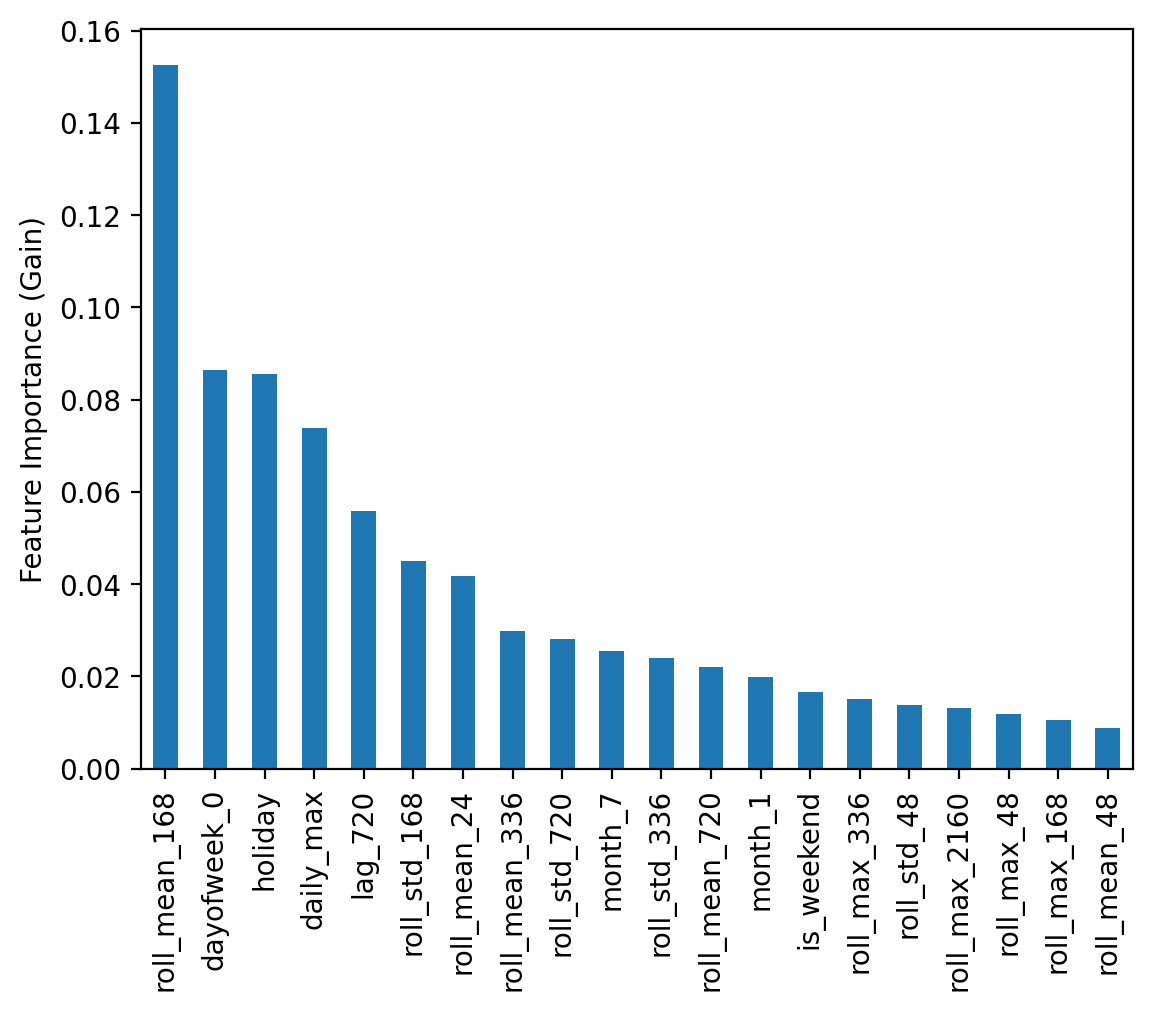
\includegraphics[width=\linewidth]{figures/feature_importance_xg.png}
	\caption{XG Boost feature importance}
	\label{fig:xg_feature_importance}
\end{figure}

Figure~\ref{fig:xg_feature_importance} shows the feature importances assigned by the model, measured by gain, which reflects how much each feature reduces the prediction error on average across all splits where it is used. The most influential feature was \texttt{roll\_mean\_168}, the rolling mean over the past week, with a gain of 0.15. This suggests that the average traffic level over the previous seven days is the single strongest predictor of the next day daily maximum. Calendar features also rank highly, with \texttt{dayofweek\_0} and \texttt{holiday} achieving gains of 0.09 and 0.09 respectively, indicating that the model has picked up on weekly rhythms and public holiday effects. Other notable features include \texttt{daily\_max} at 0.07, \texttt{lag\_720} at 0.06, and \texttt{roll\_std\_168} at 0.04, reinforcing that medium to long-term historical behaviour dominates the predictions. \\

\begin{figure}[H]
	\centering
	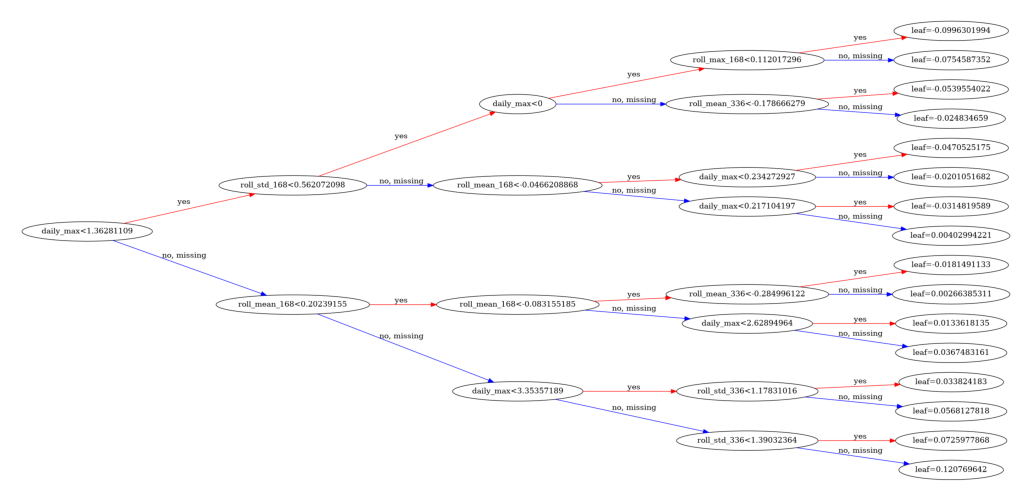
\includegraphics[width=\linewidth]{figures/xg_tree.png}
	\caption{A single tree from XG model}
	\label{fig:xg_tree}
\end{figure}

Figure~\ref{fig:xg_tree} visualises a single tree from the ensemble. At each internal node the tree makes a binary decision based on a threshold for a given feature, routing each observation either left or right until it reaches a leaf node where a prediction is made. With a maximum depth of 4, the tree can make at most 4 consecutive splits, resulting in up to 16 leaf nodes each outputting a distinct predicted value. It is worth noting that this is just one of the 200 trees that make up the final model, and on its own it is a very coarse approximation. \\

\begin{figure}[H]
	\centering
	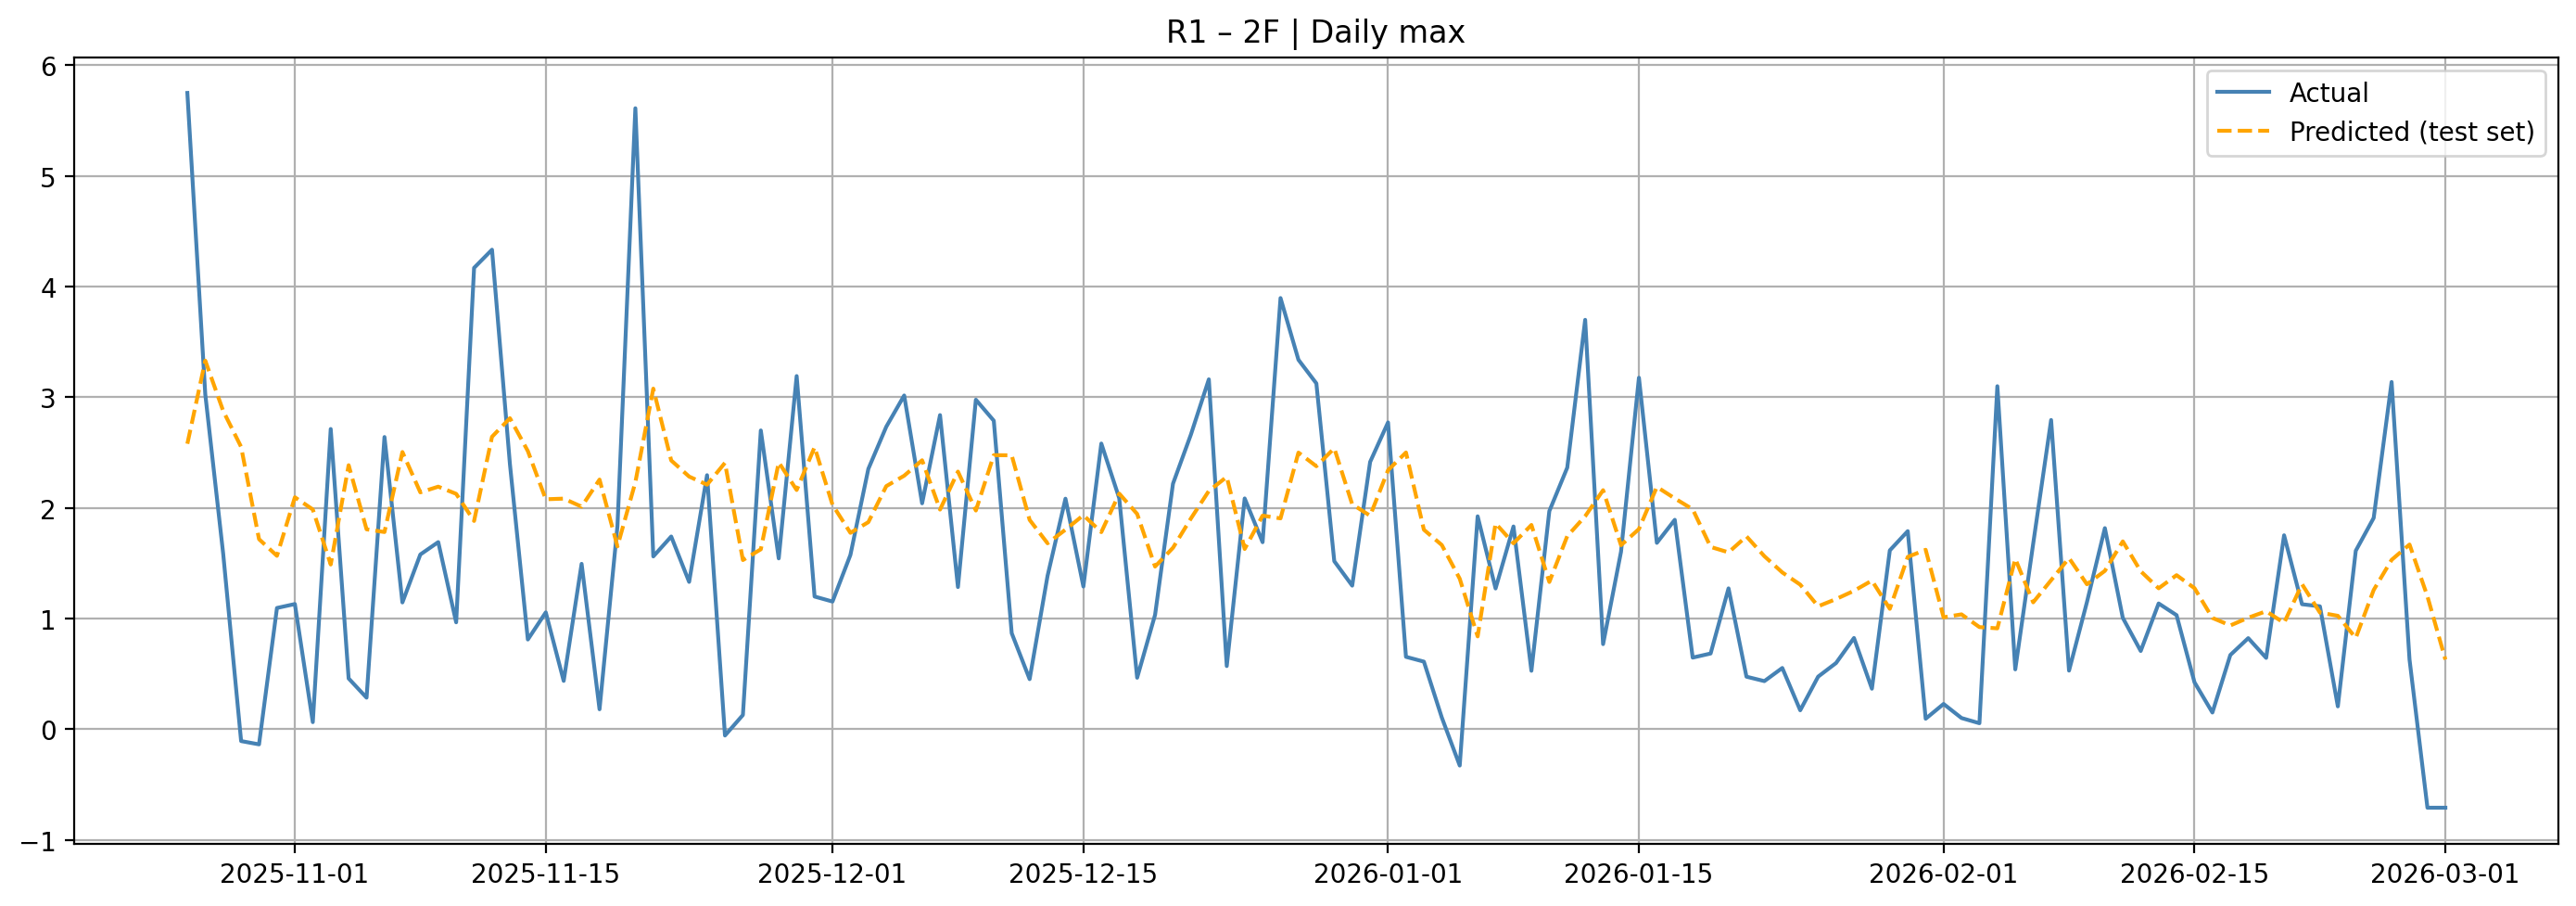
\includegraphics[width=\linewidth]{figures/xg_boost_prediction.png}
	\caption{Prediction vs Actual, xg boost on site R1 cell 2F}
	\label{fig:xg_boost_prediction}
\end{figure}

Figure~\ref{fig:xg_boost_prediction} shows the predicted versus actual daily maximum for site R1, cell 2F. The model captures the general trend and seasonal fluctuations reasonably well, though some peaks are underestimated, which is a common characteristic of tree based models that predict based on previously seen value ranges. \\

